\chapter{Introduzione}\label{chapter:introduzione} 

Durante il mio percorso presso Dieffetech, ho avuto l'opportunità di contribuire allo sviluppo e al miglioramento del gestionale interno dell'azienda.

Questo sistema rappresenta uno strumento cruciale per l’ottimizzazione dei processi aziendali e la gestione delle attività quotidiane, favorendo l’efficienza operativa e migliorando l’organizzazione interna.

\section{Dieffetech}\label{sec:cap_sec_subsec_Dieffetech}

Dieffetech S.r.l., con sede a Codogno (LO) in Via Sergio Ramelli, 24, è una dinamica software house specializzata nella creazione di soluzioni digitali personalizzate. Offre servizi di sviluppo software, siti web, applicazioni mobili e piattaforme e-commerce, mirando a soddisfare le esigenze specifiche dei clienti.

L'azienda si distingue per l'approccio consulenziale, collaborando strettamente con i clienti per sviluppare progetti e strumenti che favoriscano il successo aziendale. Tra i suoi clienti figurano realtà di rilievo come The European House – Ambrosetti, EdiliziAcrobatica, Iperal, Zucchetti e TIM Academy.

Dieffetech si impegna a fornire assistenza continua, supporto tempestivo e soluzioni innovative, garantendo prodotti testati, esteticamente gradevoli e funzionali. La sua missione è contribuire al miglioramento dei processi aziendali attraverso l'adozione di tecnologie avanzate e soluzioni digitali su misura.
\begin{figure}[H]
	\centering
	
\includegraphics[width=0.2\textwidth]{immagini/Dieffetech_logo.jpeg}
	\label{fig:dieffetech_logo}
\end{figure}
\section{Il gestionale}\label{sec:cap_sec_subsec_il_gestionale}

Il gestionale interno sviluppato da Dieffetech è una piattaforma software progettata per automatizzare e ottimizzare i principali processi aziendali. Grazie alla gestione centralizzata delle informazioni e delle attività, il sistema facilita i dipendenti nello svolgimento delle loro mansioni quotidiane.

Le sue funzionalità principali includono l’assegnazione di task giornalieri, la visualizzazione del calendario delle presenze, la gestione avanzata dei clienti, il monitoraggio dei progetti avviati e il controllo dettagliato dei costi aziendali. Queste caratteristiche rendono il gestionale uno strumento fondamentale per aumentare l’efficienza operativa, riducendo gli errori manuali e semplificando la gestione dei flussi di lavoro.
\begin{figure}[H]
	\centering
	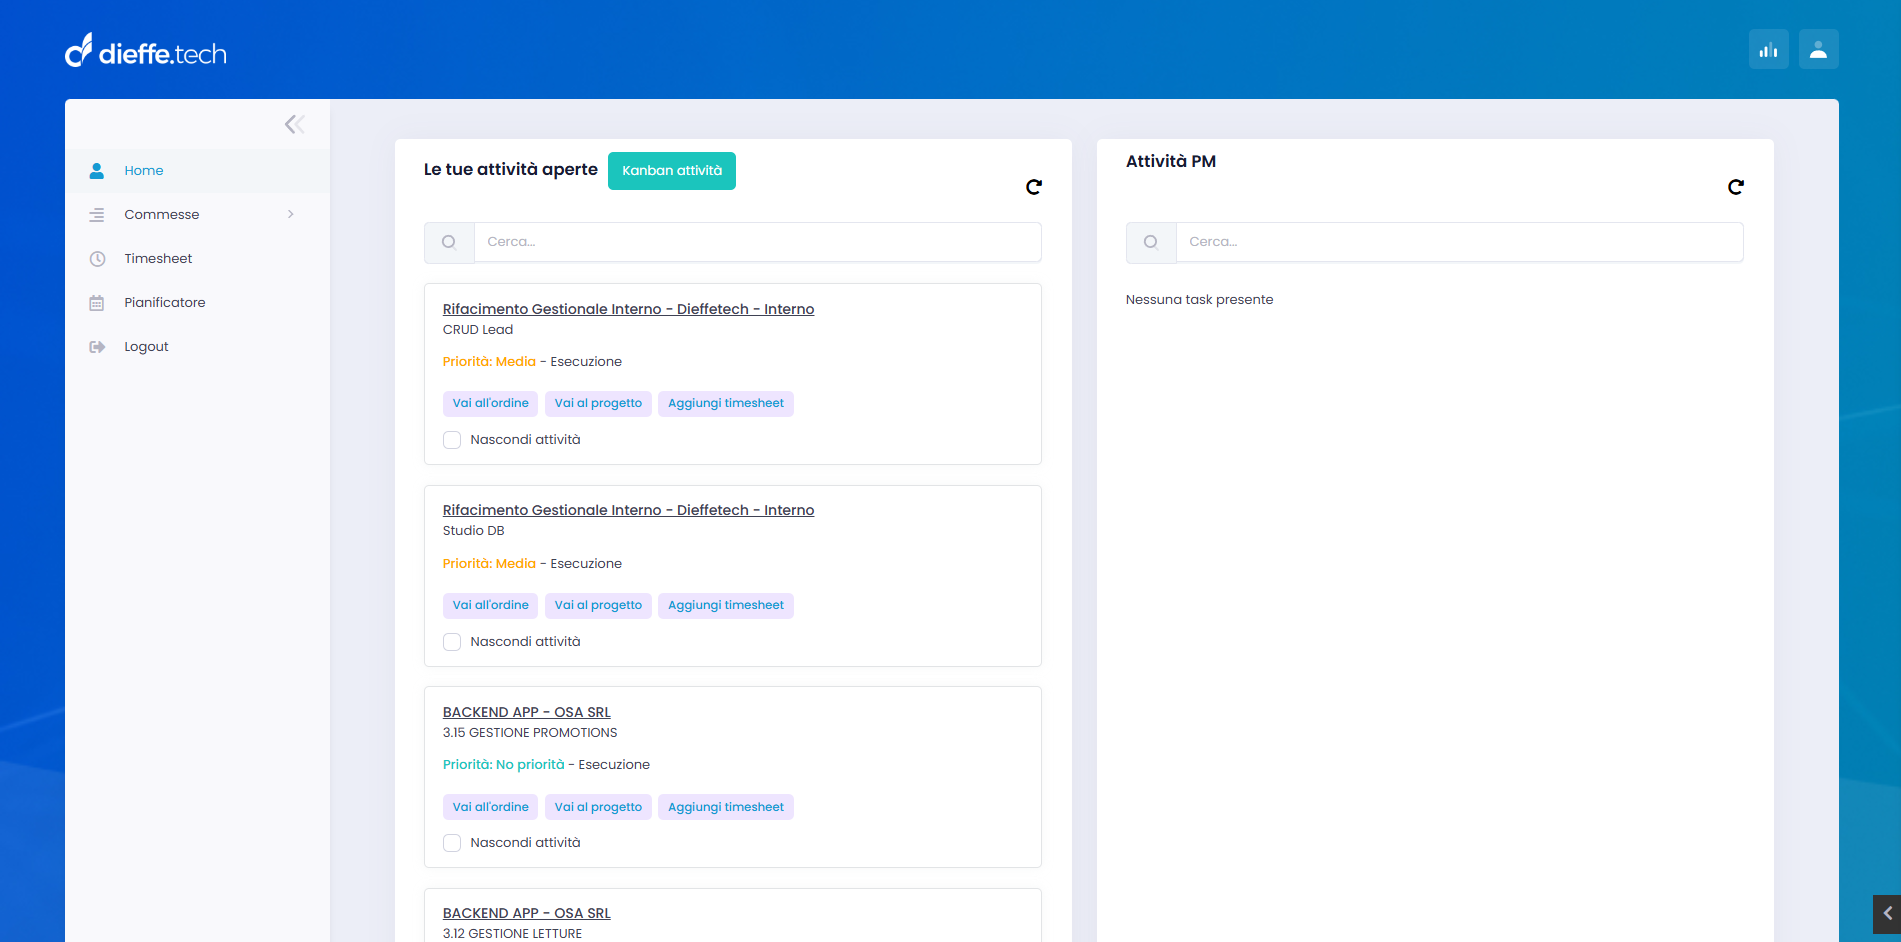
\includegraphics[width=1\textwidth]{immagini/Gesionale_Dieffetech.png}
	\label{fig:gesionale_dieffetech}
\end{figure}
\pagebreak
\section{Architettura di un'applicazione}\label{sec:cap_sec_subsec_architecture}

\begin{figure}[H]
	\centering
	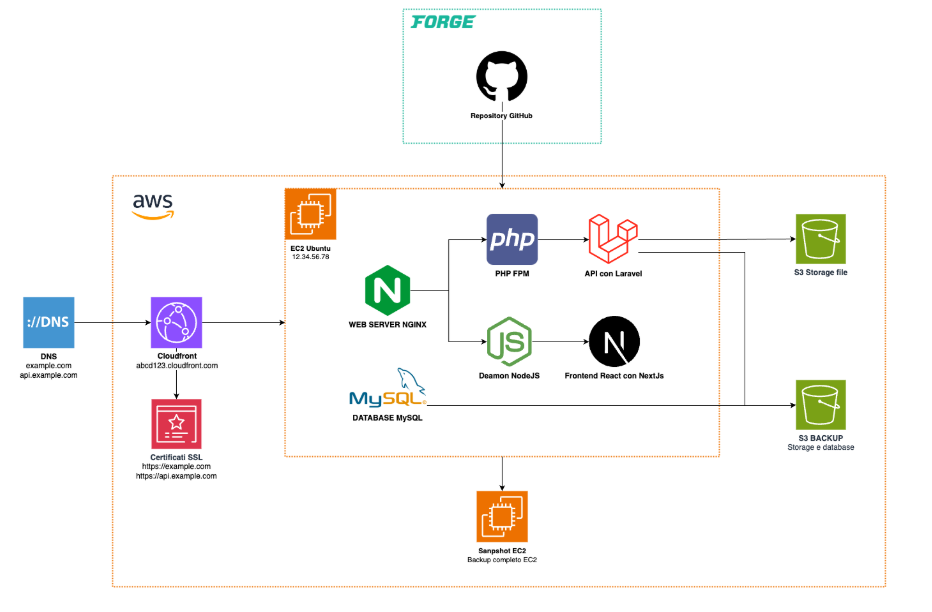
\includegraphics[width=1\textwidth]{immagini/DieffetechProjectStructure.png}
	\label{fig:project_architecture}
\end{figure}
L'architettura di un'applicazione in Dieffetech è ospitata su AWS, progettata per garantire alte prestazioni, sicurezza e scalabilità. I principali componenti e servizi utilizzati sono:

\begin{itemize}
    \item \textbf{Gestione dei DNS}: I domini \texttt{example.com} e \texttt{api.example.com} sono gestiti tramite provider DNS come Register o Aruba. I record CNAME sono configurati per puntare a AWS CloudFront, che funge da firewall per proteggere l'applicazione da attacchi DDoS, SQL Injection e Bot. Per poter usare i domini assieme a AWS CloudFlare è indispensabile l'uso di certificati SSL (https) di AWS Certificate Manager.
 
    \item \textbf{Server}: L'applicazione è ospitata su un'istanza EC2 con sistema operativo Ubuntu. La sicurezza dell'istanza è garantita da un Security Group che limita l'accesso alle porte:
    \begin{itemize}
        \item HTTP (porta 80)
        \item HTTPS (porta 443)
        \item SSH (porta 22), limitata a IP specifici
        \item MySQL (porta 3306), limitata a IP specifici
    \end{itemize}
    
    \item \textbf{Web Server}: Il server web utilizzato è Nginx, che gestisce le richieste provenienti da AWS CloudFront. Le richieste vengono poi inoltrate al frontend basato su Next.js e alle API implementate con Laravel.

    \item \textbf{Database e Storage}: Il database principale è MySQL, scelto per la sua robustezza e affidabilità. Per lo storage, viene utilizzato il disco locale dell'istanza EC2 per dati temporanei e AWS S3 per dati durevoli e scalabili.

    \item \textbf{Backup}: Sono adottate due strategie di backup per garantire la sicurezza dei dati:
    \begin{itemize}
        \item Snapshot EC2: Backup giornalieri dell'istanza EC2 per garantire un rapido ripristino in caso di guasto.
        \item Backup S3: Backup regolari dei dati e del database su AWS S3 per proteggere i dati a lungo termine.
    \end{itemize}
    
    \item \textbf{Deploy}: Il codice sorgente è gestito tramite GitHub e distribuito automaticamente su EC2 tramite Forge. Questo flusso di lavoro automatizzato riduce i tempi di deploy e gli errori manuali, assicurando una distribuzione rapida e sicura delle nuove versioni dell'applicazione.
\end{itemize}